%\section{Aikaisempi tutkimus}
\section{Mobile communications}
\label{sec:mobile_com}

\begin{itemize}
\item[--]Puhelinantennien kehitys
\item[--]Verkkotekniikat ja niiden vaatimukset
\item[--]Nykypäivän vaatimukset
\end{itemize}

\subsection{Wireless communications \& radio channel}
\label{sec:wireless_channel}
Wireless communications is often associated to mobile phones and cellular telephony or to Wireless Local Area Networks (WLAN), but the number of applications is much larger. These two examples of wireless systems may have improved everyday lives the most. Mobility of people is not anymore an obstacle of communicating with one another. Also many other useful, though not so obvious, applications have been developed. Radio Frequency Identification (RFID) is used in e.g.\ parcel tracking and keycards, satellite systems enable broadcasting over large areas and wireless sensor networks are used in monitoring. \cite{molisch}

Regardless the wireless system, whether it is satellite communications, RFID or cellular phones, the same physical principles apply. Wireless communication can be defined as transmitting and receiving information by exploiting electromagnetic spectrum and propagation of electromagnetic waves. The area between transmitter and receiver is called channel, and is illustrated in Figure \ref{fig:com_link} below. In channel the radio wave undergoes fading processes, that affect the signal strength and quality. \cite{saunders}

\begin{figure}[H]
    \centering
    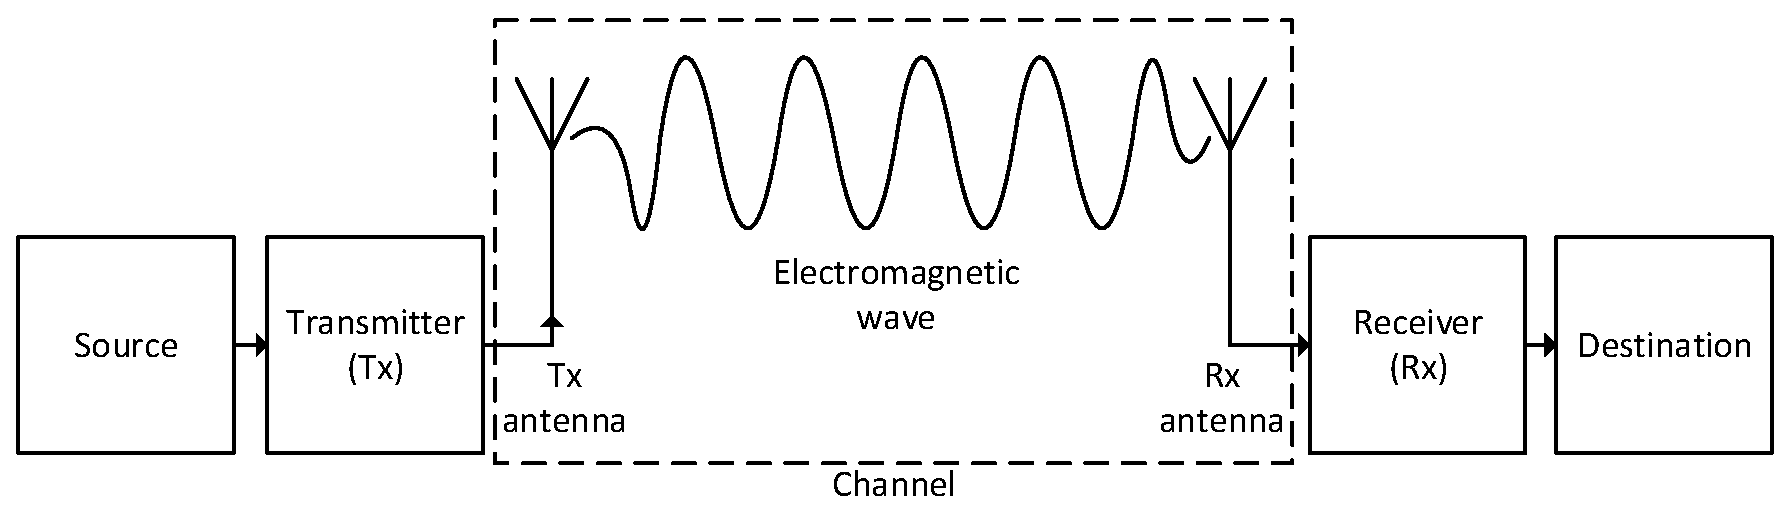
\includegraphics[width=\textwidth]{img/com_link.eps}
    \caption{Simple communication link.}
    \label{fig:com_link}
\end{figure}

\subsection{Mobile networks}
\label{sec:networks}

fsda fasdf df d \cref{sec:gsm,sec:3g,sec:lte}.

\subsubsection{Global System for Mobile communications}
\label{sec:gsm}
In 1982 the European Conference of Postal and Telecommunications Administrations (CEPT) founded the Groupe Spécial Mobile (GSM). Its purpose was to develop a new digital mobile communication system.  The new system had two requirements. First, it had to be efficient and technically better than previous wireless communication systems. It was clear at that time that analog systems would lack in user capacity, ease of use and number of additional services compared to digital system. Second, the previous analog systems were incompatible in different countries, so the new system should be standardized for whole Europe. \cite{molisch}

Developing GSM was a long process. Multiple proposals were developed by different companies. Proposals had covered nearly all possible technical solutions. Every proposed system was tested both in field and with a channel simulator. The decision was not made only based on technical aspects: also marketing and politics had influence. For example, for multiple access scheme, only Time Division Multiple Access (TDMA) was suitable. Signal processing needed for Code Division Multiple Access (CDMA) would have cost too much and was unreliable at the time. Frequency Division Multiple Access (FDMA) required antenna diversity at the mobile terminal. This would have been feasible but would have increased antenna sizes which was not desirable. However, the final developed TDMA system was a compromise. Reasons for this were political: standardizing one company's proposal would have given them a great competitive advantage. \cite{molisch}

First GSM systems were implemented in Europe after 1992. Soon it was realized that functionalities that originally had not been included in the standard were needed. These were developed by 1995. Later, General Packet Radio Service (GPRS) and the more efficient modulation of Enhanced Data rates for GSM Evolution (EDGE) have been included. \cite{molisch}
%%Lisää GPRS & EDGE data ratet vrt. alkuperäinen

GSM is the most successful mobile communication system worldwide. It had spread from Europe to all over the world, except Japan and Korea, where it was never implemented. Since GSM was now a worldwide standard, it was renamed Global System for Mobile communications. \cite{molisch}

GSM operates at three different carrier frequencies. Original systems use frequencies around 900\,MHz. Number of subscriptions increased which led to the addition of 1800\,MHz band. That band has more or less three times more bandwidth available than the original carrier. The new band also increased network capacity significantly. Third system operating at 1900\,MHz band is mainly used in the United States.  Table \ref{tab:gsm} below presents the key specifications and differences of the three versions of GSM. \cite{molisch}

\begin{table}[H]
    \centering
    \caption{Specifications of GSM carriers.} %lähde
    \label{tab:gsm}
    \begin{tabular}{|c|c|c|c|c|}
        \hline
         Carrier & Uplink frequency & Downlink frequency & Bandwith & Data rate \\%vai Capacity
         \hline
         GSM900 & 880-915\,MHz & 925-960\,MHz & & \\
         \hline
         GSM1800 & 1710-1785\,MHz & 1805-1880\,MHz & & \\
         \hline
         GSM1900 & 1850-1910\,MHZ & 1930-1990\,MHz & & \\
         \hline
    \end{tabular}
\end{table}

\subsubsection{Third generation mobile networks}
\label{sec:3g}
The success beyond expectations of GSM inspired the development of a new communication system. International Telecommunications Union (ITU) announced few goals for a standard called International Mobile Telecommunications (IMT-2000) for the third generation (3G) mobile communication system. The new system should have better performance, meaning better spectral efficiency and higher peak data rates: 2\,Mb/s indoor and 348\,kb/s outdoor. Same time, channel bandwidth should increase from 200\,kHz to 5\,MHz. Also new multimedia applications should be supported, which would require flexibility in choosing the data rates. Finally, the system should be backwards compatible with GSM. \cite{molisch}

In early 1990s, different European groups developed proposals for 3G within the European Telecommunications Standards Institute (ETSI). Proposed solutions ranged from TDMA and CDMA to new Orthogonal Frequency Division Multiplexing (OFDM). In 1998 two drafts were selected to form the European proposal for the new network standard: Wideband Code Division Multiple Access (WCDMA). First draft defined a Frequency Division Duplexing (FDD) mode which operates as the basic system. Second introduced a Time Division Duplexing (TDD) mode which supported high data rate applications. WCDMA usually refers to the radio access technology, and the complete 3G network is called Universal Mobile Telecommunication System (UMTS). \cite{molisch}

Europeans were not the only ones making proposals for the IMT-2000 family. Japanese also proposed a WCDMA system that was rather similar to the European, and thus merged. Besides the Europe-Japan collaboration, four other proposals had strong support, which made reaching an agreement for a single 3G system impossible within the ITU. As a compromise, ITU decided to declare all proposals as different modes of IMT-2000. Later Time Division Synchronous Code Division Multiple Access (TD-SCDMA) was an important part of 3G developments and then accepted to the IMT-2000 family. \cite{molisch}

The European/Japanese standard was further developed by the Third Generation Partnership Project (3GPP). Newer versions of the standard included improvements, such as High-Speed Packet Access (HSPA). It was first implemented for downlink and later realized for uplink also. Different UMTS technologies are compared in the table \ref{tab:3g} below. \cite{molisch} %%Täytä taulukko WCDMA vs TD-SCDMA vs HSPA %%kerro tekstissä taajuudet jne teknistä dadaa.

\begin{table}[H]
    \centering
    \caption{Comparison of different 3G technologies.} %lähteet
    \label{tab:3g}
    \begin{tabular}{|c|c|c|c|}
         \hline
         Standard &  Frequencies & Bandwidth & Peak data rate\\
         \hline
         WCDMA & & &\\
         \hline
         TD-SCDMA & & &\\
         \hline
         HSPA & & &\\
         \hline
    \end{tabular}
\end{table}

The number of different specifications had grown so much that it was a problem for 3GPP. Increased costs and delays in time to market nearly killed 3G. First UMTS networks were planned to start operating in 2002, but it took off only around 2005. Besides technical problems also lack of applications requiring high data rates in the market delayed the implementation. By 2009 these problems were solved and UMTS had become successful all around the world. \cite{molisch}

\subsubsection{Long-Term Evolution}
\label{sec:lte}
While WCDMA was being deployed and spreading out, 3GPP started to research a new, fourth generation (4G) network system. They supposed that data rates and spectral efficiencies of WCDMA would not be sufficient for the future applications and demands. The new standard was named Long-Term Evolution (LTE) and it was constructed from a scratch and differences to previous standards were significant. LTE uses Orthogonal Frequency Division Multiple Access (OFDMA) scheme, OFDM modulation and has a limited support for Multiple Input Multiple Output system (MIMO) antenna technology. Also its core network is purely packet-switched while GSM was circuit-switched and 3G a combination of the two. \cite{molisch}

For 4G network standard, IMT-Advanced, ITU announced requirements in 2008. Such systems should provide access to advanced mobile services and have capabilities for high quality multimedia applications. The performance requirements included better spectral efficiency, scalable bandwidth up to at least 40\,MHz and peak data rates of 1\,Gb/s. \cite{itur} However, LTE has peak data rate of 300\,Mb/s, which is not fulfilling the IMT-Advanced standard. Further development have extended the use of MIMO for better spectral efficiency. Newer release called LTE-Advanced is promising 1\,Gb/s peak data rates and is one candidate for IMT-Advanced cellular system. \cite{molisch} %%viittaus taulukkoon alla, täytä taulukko

\begin{table}[H]
    \centering
    \caption{LTE and LTE-Advanced fulfillment of IMT-Advanced \cite{parkvall_lte}.}
    \label{tab:lte}
    \begin{tabular}{|l|M{3cm}|M{3cm}|M{3cm}|}
        \hline
         & IMT-Advanced requirement & LTE & LTE-Advanced \\
        \hline
        Peak data rate & & & \\
        -Downlink & & & \\
        -Uplink  &  & & \\
        \hline
        Spectral efficiency & & & \\
        -Downlink & 15\,b/s/Hz & 16\, b/s/Hz & 16\, b/s/Hz*\\
        -Uplink  & 6.75\, b/s/Hz & 4\, b/s/Hz & 8.1\, b/s/Hz**\\
        \hline
        Bandwidth & At least 40\,MHz & Up to 20\,MHz & Up to 100\,MHz \\
        \hline
    \end{tabular}
    
    *For 4x4 MIMO antenna system. 8x8 could reach 30\,b/s/Hz.\\
    **For 2x2 MIMO antenna system. 4x4 could reach 16.1\,b/s/Hz.
\end{table}

4G systems should be backwards compatible with 3G and GSM. Also the transitions from older technology to newer one should be smooth, which requires two system to coexist and use the same frequency bands. LTE and LTE-Advanced operate on a number frequency bands. Due to the national frequency regulators, all bands are not available in all countries. Since some frequencies are already allocated to e.g.\ WCDMA or GSM, corresponding frequency bands are created and operators are anticipated to migrate. All frequency bands are listed in table \ref{tab:lte_bands} below. \cite{molisch, radio_electronics}

\begin{table}[H]
    \centering
    \caption{LTE frequency band allocation for FDD and TDD modes. \cite{radio_electronics}}
    \label{tab:lte_bands}
    \begin{tabular}{|c|c|c|}
        \hline
        \multicolumn{3}{|c|}{FDD bands} \\
        \hline
         Band & Uplink (MHz) & Downlink (MHz) \\
         \hline
         1 & 1920 - 1980 & 2110 - 2170\\
         \hline
         2 & 1850 - 1910 & 1930 - 1990\\
         \hline
         3 & 1710 - 1785 & 1805 - 1880\\
         \hline
         4 & 1710 - 1755 & 2110 - 2155\\
         \hline
         5 & 824 - 849 & 869 - 894\\
         \hline
         6 & 830 - 840 & 875 - 885\\
         \hline
         7 & 2500 - 2570 & 2620 - 2690\\
         \hline
         8 & 880 - 915 & 925 - 960\\
         \hline
         9 & 1749.9 - 1784.9 & 1844.9 - 1879.9\\
         \hline
         10 & 1710 - 1770 & 2110 - 2170\\
         \hline
         11 & 1427.9 - 1452.9 & 1475.9 - 1500.9\\
         \hline
         12 & 698 - 716 & 728 - 746\\
         \hline
         13 & 777 - 787 & 746 - 756\\
         \hline
         14 & 788 - 798 & 758 - 768\\
         \hline
         15 & 1900 - 1920 & 2600 - 2620\\
         \hline
         16 & 2010 - 2025 & 2585 - 2600\\
         \hline
         17 & 704 - 716 & 734 - 746\\
         \hline
         18 & 815 - 830 & 860 - 875\\
         \hline
         19 & 830 - 862 & 791 - 821\\
         \hline
         20 & 832 - 862 & 791 - 821\\
         \hline
         21 & 1447.9 - 1462.9 & 1495.5 - 1510.9\\
         \hline
         22 &  3410 - 3500 & 3510 - 3600\\
         \hline
         23 & 2000 - 2020 & 2180 - 2200 \\
         \hline
         24 & 1625.5 - 1660.5 & 1525 - 1559\\
         \hline
         25 & 1850 - 1915 & 1930 - 1995\\
         \hline
         26 & 814 - 849 & 859 - 894\\
         \hline
         27 & 807 - 824 & 852 - 869\\
         \hline
         28 & 703 - 748 & 758 - 803\\
         \hline
         29 & downlink only & 717 - 728 \\
         \hline
         30 & 2305 - 2315 & 2350 - 2360\\
         \hline
         31 & 452.5 - 457.5 & 462.5 - 467.5\\
         \hline
         \hline
         \multicolumn{3}{|c|}{TDD bands} \\
         \hline
         Band & \multicolumn{2}{|c|}{Allocation (MHz)}\\
         \hline
         33 & \multicolumn{2}{|c|}{1900 - 1920}\\
         \hline
         34 & \multicolumn{2}{|c|}{2010 - 2015}\\
         \hline
         35 & \multicolumn{2}{|c|}{1850 - 1910 }\\
         \hline
         36 & \multicolumn{2}{|c|}{1930 - 1990 }\\
         \hline
         37 & \multicolumn{2}{|c|}{1910 - 1930 }\\
         \hline
         38 & \multicolumn{2}{|c|}{2570 - 2620}\\
         \hline
         39 & \multicolumn{2}{|c|}{1880 - 1920 }\\
         \hline
         40 & \multicolumn{2}{|c|}{2300 - 2400}\\
         \hline
         41 & \multicolumn{2}{|c|}{2496 - 2690 }\\
         \hline
         42 & \multicolumn{2}{|c|}{3400 - 3600 }\\
         \hline
         43 & \multicolumn{2}{|c|}{3600 - 3800}\\
         \hline
         44 & \multicolumn{2}{|c|}{703 - 803}\\
         \hline
    \end{tabular}
\end{table}

\clearpage
